\documentclass[a4paper,11pt]{article}
\usepackage[T1]{fontenc}
\usepackage[utf8]{inputenc}
\usepackage{lmodern}
\usepackage{hyperref}
\usepackage[top=2cm, bottom=2cm, left=2cm, right=2cm]{geometry}
\usepackage{graphicx}
\usepackage{listings}
\usepackage{color}
\usepackage{amsmath}
\usepackage{mathtools}
\usepackage{tikz}
\usepackage{subcaption}
\usepackage{tcolorbox}
\usepackage{rotating}

\title{Implementation of a compiler for an imperative language\\IMP}
\author{Remy Detobel \& Denis Hoornaert}

\newcommand{\subsubsubsection}[1]{\paragraph{#1}\mbox{}\\}
\setcounter{secnumdepth}{4}
\setcounter{tocdepth}{4}

% For tikz purposes
\tikzset{% 
  tree/.style = {
    sibling distance=5em,
    every node/.style = {shape=rectangle, rounded corners,
      draw, align=center,
      top color=white, bottom color=blue!20},
    edge from parent/.style = {draw,-latex}
  }
}

\definecolor{codegreen}{rgb}{0,0.6,0}
\definecolor{codegray}{rgb}{0.5,0.5,0.5}
\definecolor{codepurple}{rgb}{0.58,0,0.82}
\definecolor{backcolour}{rgb}{0.95,0.95,0.92}
 
\lstdefinestyle{mystyle}{
    backgroundcolor=\color{backcolour},   
    commentstyle=\color{codegreen},
    keywordstyle=\color{magenta},
    numberstyle=\tiny\color{codegray},
    stringstyle=\color{codepurple},
    basicstyle=\footnotesize,
    breakatwhitespace=false,
    breaklines=true,
    captionpos=b,
    keepspaces=true,
    numbers=left,
    numbersep=5pt,
    showspaces=false,
    showstringspaces=false,
    showtabs=false,
    tabsize=2
}
 
\lstset{style=mystyle}

\begin{document}

\maketitle
\tableofcontents

\newpage

\section{Introduction}

  The aim of project is to implement a compiler for a 'simple' imperative language named \textit{IMP}. Like any imperative programming language, \textit{IMP} is composed of mainstream features such as \textit{keywords} (\verb|if|, \verb|while|, ... statements), \textit{variables}, \textit{numbers} and \textit{comments}.
  The form of these features follows some defined rules~:
  \begin{itemize}
    \item a \textit{variable} is a sequence of alphanumeric characters that must start by a letter.
    \item a \textit{number} is a sequence of one or more digits.
    \item a \textit{comment} must start by the combination '\verb|(*|' and ends by the reversed combination '\verb|*)|'. 
  \end{itemize}
  The compilation scheme is generally divided in three main phases~: analysis, synthesis and optimisation. The phases are themselves composed of different steps. For instance, the analysis phase is composed of \textit{lexical analysing} step (or \textit{scanning}), a \textit{syntax analysing} step (or \textit{parsing}) and a \textit{semantic analysing} step as shown in fig.\ref{compilation_phases}. In this assignment, the focus is set on the \textit{analysis phase}.
  \begin{figure}[h]
    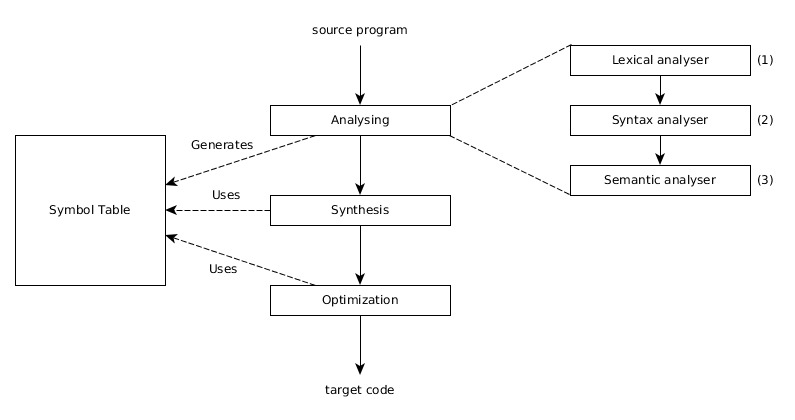
\includegraphics[scale=0.45]{./img/phase_of_compiler.jpg}
    \centering
    \caption{Compilation phases}
    \label{compilation_phases}
  \end{figure}
  
\section{Implementation of the lexical analyser}
  In the so called "Dragon book"\footnote{V. Aho, A., 2007. \textit{Compilers~: Principles, techniques, \& Tools.} 2nd ed. New York~: Pearson.} the \textit{lexical anlyser} is defined as follow~:
  \begin{center}
    <<The \textit{lexical analyser} reads the stream of characters making up the source program and groups the characters into a meaningful sequence called \textit{lexemes}.>>
  \end{center}
  A \textit{lexeme} can be defined as a tuple which contains both a \textit{token name} and the associated value (not always mandatory). The sequence of \textit{lexemes} generated by the \textit{lexical analyser} will be used by the following step. In addition, the \textit{lexical analyser} will generate a very useful tool used during all the other steps (as shown in fig.\ref{compilation_phases} .) and called a \textit{symbol table}. The role of the \textit{symbol table} is to store every variable encountered while scanning the source code and the line where it appears for the first time.\\
  
  \subsection{Use of a lexical analyser generator}
    In order to ease the process of recognizing the lexemes defined in the given \verb|LexicalUnits.java| file many \textit{lexical analysers} have been developed. Among them, the most well known generator is the flex program and all its derived versions. In the present project, \verb|jflex| is used as it has been decided to implement the project using the \verb|java| programming language. Using a \textit{lexical analyser generator} eases the analysis of any input because it enables the programmers to describe every \textit{regular expression} by using the \textit{Regex} writing convention and then to generate a \verb|.java| file that will recognise all of them. This generated \verb|.java| file can then be used as any other \verb|java| class.
    \begin{figure}[h]
      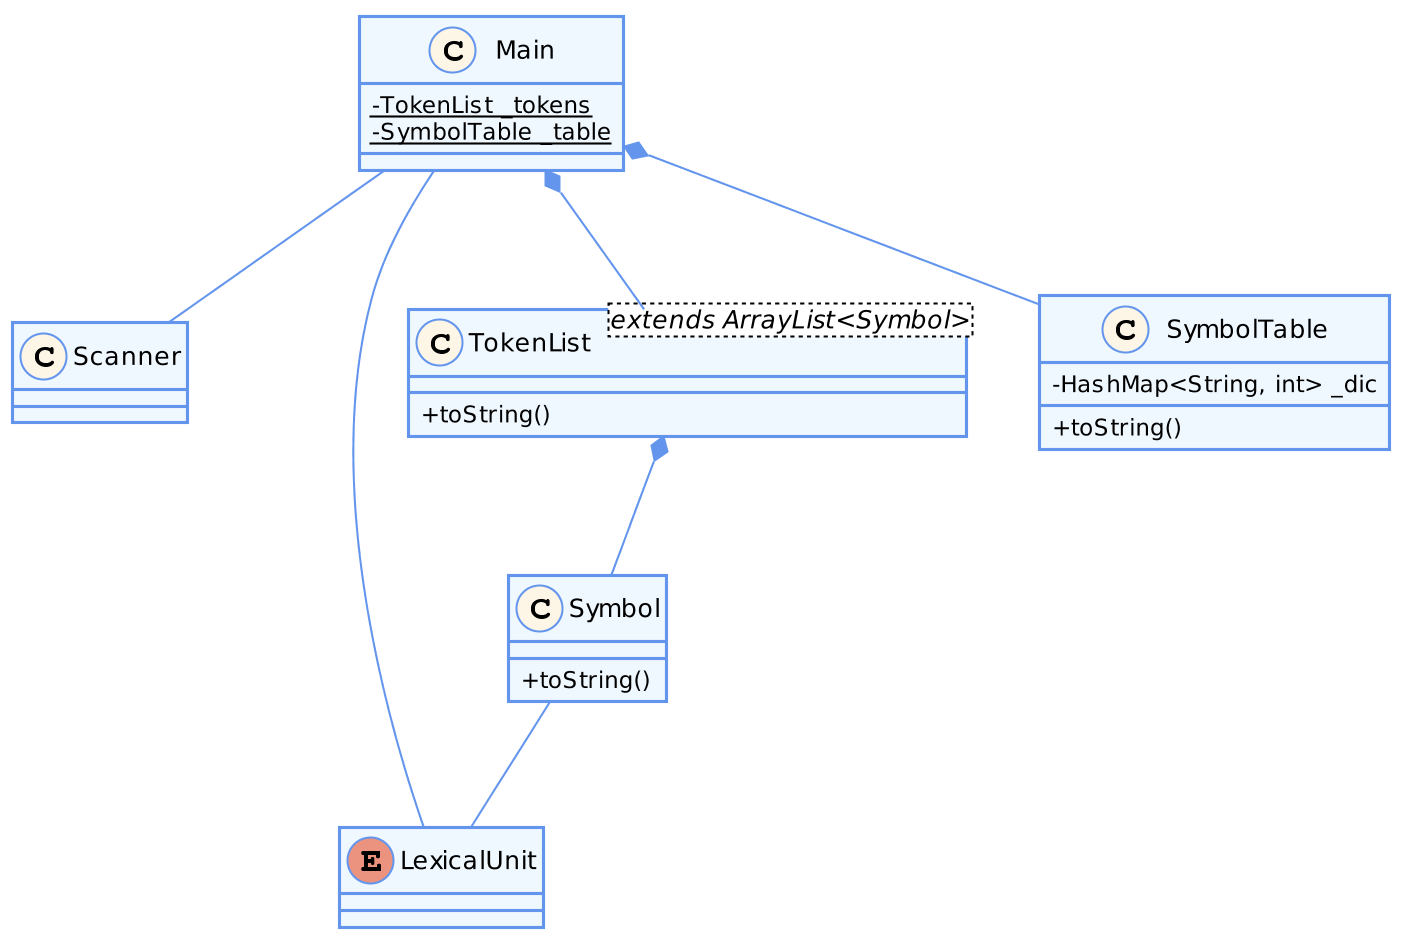
\includegraphics[scale=0.15]{./img/class_diag.png}
      \centering
      \caption{Model class (Pseudo-UML). The TokenList class is the sequence of lexemes and the Scanner class is the file generate by jflex}
    \end{figure}
  
  \subsection{Regular expressions}
    Based on the content of \verb|LexicalUnits.java|, we can easily divide the set of lexical units into two distinct groups~: the \textit{keyword} group and the variable/constant group.\\
    The implementation of the \textit{keyword} group using regular expressions is pretty straightforward as simply writing the \textit{keyword} is sufficient. For instance, the regular expression of the \textit{keyword} \verb|if| is simply \verb|if|.\\
    On the other hand, the implementation of the variable/constant group requires slightly more work. This small group is composed of two elements the variables and the numbers.\\
    The structure of \textit{variables} given in the assignment statements is "a sequence of alphanumeric characters that must start by a letter". Thus, the equivalent regular expression is~:
    \begin{verbatim}
[a-zA-Z][a-zA-Z0-9]*
    \end{verbatim}
    The structure of \textit{numbers} given in the assignment statements is "a sequence of one or more digits". thus, the equivalent regular expression is~:
    \begin{verbatim}
[0-9]+
    \end{verbatim}
  
  \subsection{Hypothesis on regular expressions}
    \label{hypothesis}
    The only hypothesis that has been made throughout the realisation of the project concerns the behaviour of the \textit{lexical analyser} when a character not specified in either the structure of a \textit{number}, a \textit{variable} or a \textit{keyword} is encountered. Typically, amongst this set there are the following characters~:
    \begin{center}
      \verb|}|, \verb|{|, \verb|_|, \verb=|=, \verb|&|, \verb|[|, \verb|]|, \verb|(|, \verb|)|
    \end{center}
    In order words, the question is~: What does the \textit{lexical analyser} do for the following line~:
    \begin{lstlisting}
index_of_loop := list[x]\end{lstlisting}
    Four ideas have been considered~:
    \begin{itemize}
      \item Considering these characters as a new lexical unit identified by the following regular expression (not exhaustive)~:
        \begin{verbatim}
SpecialChar = ["}", "{", "_", "|", "&", "[", "]", "(", ")"]
        \end{verbatim}
        The example above would be transposed by the \textit{lexical analyser} into the following token list~:
        \begin{verbatim}
token: index              lexical unit: VARNAME
token: _                  lexical unit: SPECIALCHAR
token: of                 lexical unit: VARNAME
token: _                  lexical unit: SPECIALCHAR
token: loop               lexical unit: VARNAME
token: :=                 lexical unit: EQUAL
token: [                  lexical unit: SPECIALCHAR
token: x                  lexical unit: VARNAME
token: ]                  lexical unit: SPECIALCHAR
        \end{verbatim}
        Unfortunately, the assignment statement disallows us to modify the \verb|LexicalUnits.java| file. Consequently, this possibility is not relevant.
      \item Considering these characters as normal characters. This would mean that they could be part of a \textit{variable} name. Thus, the regular expression for identifying \textit{variables} has to be modify to look like~:
        \begin{verbatim}
SpecialChar = ["}", "{", "_", "|", "&", "[", "]", "(", ")"]
[a-zA-Z|SpecialChar][a-zA-z0-9|SpecialChar]*
        \end{verbatim}
        As a consequence, the token list generated by the \textit{lexical analyser} will behave as follow~:
        \begin{verbatim}
token: index_of_loop      lexical unit: VARNAME
token: :=                 lexical unit: EQUAL
token: [x]                lexical unit: VARNAME
        \end{verbatim}
        Even though, using characters like \verb|_| in variable name is common in many programming languages, the other characters are generally not used for this purpose. Given this fact and the fact that the assignment statement does not explicitly mention such a possibility, this idea has been overlooked. Moreover, this implies that variable such as \verb|{{!^^§'#| would be considered as valid even though having such \textit{variables} is not handy.
      \item Not considering them. In this possibility, we just overlook them like if they were equivalent to a space character. Implementing this idea is quick but does not really make sense because theses characters would then cause many problems in the following steps.
      \item Throwing an error. This idea consists simply on printing a warning when an unexpected character is encountered and on stopping the program as resuming does not make any sense. Moreover, this behaviour is pretty common in many programming languages. This solution is the one who fits the best the assignment statements. Therefore, this solution has been preferred over the two others.
    \end{itemize}

  \subsection{Dealing with nested comments}
    The management of comments using regular language is quite simple. Once an opening statement (here : '\verb|(*|') has been encountered, it overlooks the following characters until it encounters a closing statement (here : '\verb|*)|').
    \begin{lstlisting}
(*I am a (*nested*) comment*)\end{lstlisting}
    Unfortunately, applying the same mechanism on a nested comment will result in a ill-formed outcome. Indeed, in the case of the example above, the analyser will overlook the second opening statement (columns 9 \& 10) and will stop when it comes across the first closing statement (columns 17 \& 18) having for consequence that the third part of the \textit{nested comment} will remain.\\
    To overcome this problem, the analyser must know how many opening statements it came across and how many closing statements it should expect to encounter in order to know whether it is still in a comment.\\
    The most obvious and smartest way to implement it is to use a counter (i.e. a memory) that will be incremented for every opening statement encountered and decreased for every closing statement encountered. However, from a theoretical point of view, by using a memory the language cannot be considered as regular any more. In the present project, it is not a problem and \verb|jflex| allows us to implement such a language.
    
  \subsection{Tests and results}
    \label{subsec:testscanner}
    In this section, the results of the implementation are analysed and tested throught three \textit{IMP} source codes~: one given in the assignment statements and the two others inspired by algorithms from the Syllabus of Thierry Massart\footnote{Thierry Massart, 2014. \textit{Programmation.} Release 3.3.3~.}. The aim of testing the \textit{lexical analyser} on these three tests is to ensure that a maximum of the \textit{keywords} and the \textit{variables} are recognized because the set of keywords in the \verb|Euclid.imp| (fig.\ref{code:euclid}) file does not cover every possibilities. This is why these two codes have been chosen. As explained above in the hypothesis subsection \ref{hypothesis}, the program in fig.\ref{code:sort} simply stops its execution as it encounters an undefined character at line 1 ('\verb|[|'). Unfortunately, it is difficult to cover all the different statements as finding interesting samples of code that do not use list(s) is hard.
    \begin{figure}[h!] % cacule réellement le gcd
      \lstinputlisting{../../test/imp/Euclid.imp}
      \caption{\textit{IMP} code to compute the gcd of two numbers}
      \label{code:euclid}
    \end{figure}
    \begin{figure}[h!]
      \lstinputlisting{../../test/imp/Fibonacci.imp}
      \caption{Implementation of the Fibonacci \textit{"algorithm"} using \textit{IMP}}
      \label{code:fibonacci}
    \end{figure}
    \begin{figure}[h!]
      \lstinputlisting{../../test/imp/Sort.imp}
      \caption{Implementation of a sorting algorithm using \textit{IMP}}
      \label{code:sort}
    \end{figure}
    
\section{Implementation of the syntax analyser}
  The \textit{syntax analysis} (or \textit{parsing}) is the step of the \textit{analysis} phases (see fig.\ref{compilation_phases}) that aims to verify the \textit{syntax} of the source code (under the form of a list of tokens) and to report the potential errors using a grammar (see definition later) given by the language designer.\\
  The outcome of the parser is a \textit{syntax tree} that will be used by the following phase (as shown in the fig.\ref{compilation_phases}). We distinguish two types of \textit{parsers} : the \textit{top-down} and the \textit{bottom-up}.\\
  As previously mentioned, \textit{parsers} uses a specific structure called \textit{grammar} which, similarly to spoken languages, aims to describe the allowed structures that a language can display.
  The \textit{grammar} is composed of a set of variables to which are associated at least one rule. Typically, a \textit{grammar} is written following a fixed convention (see fig.\ref{fig:unmodifiedgrammar1} or any other grammar). Generally, in the case of a programming language, \textit{context-free grammar} are used because of its user-friendly aspect and the fact that it allows an iterative development. However, \textit{context-free} grammars are not well adapted for implementation. Therefore, \textit{parser generators} usually transform them into \textit{LL(K)} grammars. In the assignment statement, it is asked to transform the IMP grammar into a \textit{LL(1)}.\\
  A LL(1) grammar is a class of grammars that can be defined by a predictive top-down parser. Such grammars define context-free languages which can be recognised by push-down automaton (i.e. automaton that use a stack as memory). We define a predictive parser as a type of parser that has an access to the input (other than read). This access is characterised by the possibility to know what is the following character to be read (this is very different from reading on the input) in order to enable the parser to take deterministic decisions throughout its execution.
  
  \begin{figure}[h!]
    \centering
    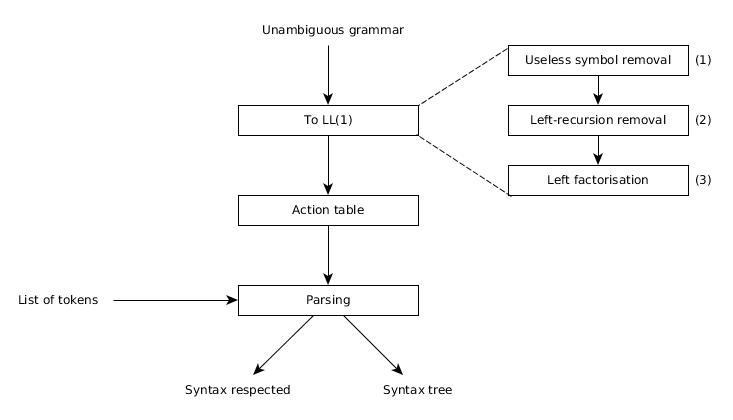
\includegraphics[scale=0.45]{./img/phase_of_parsing.jpg}
    \caption{Phases of a parser generator}
    \label{fig:parsergeneratorphases}
  \end{figure}
  
  \subsection{Use and implementation of a parser generator}
  Nowadays, when designing a programming language, one might find convenient to use a program dedicated to the determinisation of the grammar and the \textit{parse tree} generation. Such programs are well known and have been developed a long time ago (e.g. yacc in the 1970's).\\
  However, the assignment statement does not allow the use of such a program. Henceforth, it has been decided to implement a dedicated \textit{parser generator} so that the given grammar will be modified without suffering from possible human mistakes. All the steps that a \textit{parser generator} must achieved are shown in the fig.\ref{fig:parsergeneratorphases} and explained the section \ref{grammartoll1methods}.
  
  \subsection{Parser phases}
    The present section is divided in three subsections each explaining the utility of the different mechanisms that composes a \textit{parser generator}. The first subsection concerns the transformation of a \textit{context-free} grammar into an \textit{LL(1)} grammar, the second subsection focuses on the creation of an \textit{action table} and the last subsection explains how to check the syntax of an input.\\
    A reader aware of the mechanisms used can easily skip the present section and resumes at the results section (\ref{sec:results}).
  
    \subsubsection{Transforming the grammar into an LL(1) grammar}
      \label{grammartoll1methods}
      In order to transform a given grammar that can be either deterministic or non-deterministic into a LL(1) --- which is deterministic ---, one must apply four transformations on this grammar. These transformations aim to make the grammars deterministic and thus implementable.
      \begin{description}
        \item[Ambiguity removal~:] Consists of ensuring, by the introduction of rule layers, that for a same input only one interpretation/derivation is possible. It also allows to force and to fix the priority and the associativity of some terminals in the grammar. (For further explanations see annex~\ref{sec:ambiguity})
        \item[Useless variable removal~:] Consists of removing every variable that does not appear in any other rule of the grammar (as they will never be called/used) and removing variable that does not contain a rule capable of stopping the recursion of the other rules of the same variable. (For further explanations see annex~\ref{sec:useless})
        \item[Left-recursion removal~:] Consists of modifying every rules where the recursion occurs at the first element so that a grammar can still accept non-finite languages but becomes deterministic because the parser will eventually always encounter a terminal. (For further explanations see annex~\ref{sec:leftrecursion})
        \item[Left-factorisation~:] Consists of finding every rules of a variable that have a common prefix (i.e. same sequence of tokens) and of modifying it in consequence so that the parser can take deterministic decision. For example~: which rule to choose between $S \rightarrow \alpha A$ and $S \rightarrow \alpha Z$ when the look ahead is $\alpha$. (For further explanations see annex~\ref{sec:factorisation})
      \end{description}
  
    \subsubsection{Action table}
      \label{subsubsec:actionTable}
      An action table is a structure that emphasises the relation between a given variable and a terminal. Actually, it helps answering the following question : Which rule of a variable has to be applied if the next symbol to be read is x ?\\
      To construct this structure, one has to introduce the function $first(\alpha)$ that returns all the symbols that can be reached in one step (i.e. using only the first element of a rule). If the first element of the rule is a terminal, $first(\alpha)$ adds this terminal to the returned set (the set of reachable variables). Otherwise, if the element is a variable, it calls $first(\alpha)$ on it and then merges the returned set with the current one. Unfortunately, there is a special case : the epsilon-rule\footnote{a variable rule which is only composed of an epsilon ($\epsilon$)}. In fact, because $\epsilon$ is neither a variable or a terminal and is --- by definition --- not expected on the input, one must, when encountering an epsilon, apply the function $first(\alpha)$ on any element following an appearance of the variable that owns the epsilon-rule. The research of those elements is done by a function called $follow(\alpha)$.
      \begin{figure}[h!]
        \centering
        \begin{subfigure}[b]{0.4\textwidth}
            \centering
            \begin{align}
              S &\rightarrow aAcCa \\
              A &\rightarrow Sc \\
              A &\rightarrow \epsilon \\
              C &\rightarrow c
            \end{align}
            \caption{Grammar}
            \label{fig:simplegrammar}
        \end{subfigure}
        \begin{subfigure}[b]{0.4\textwidth}
            \centering
            \begin{tabular}{|c||c|c|}
              \hline
                & a & c \\
              \hline
              \hline
              S & 1 &   \\
              \hline
              A & 2 & 3 \\
              \hline
              C &   & 4 \\
              \hline
            \end{tabular}
            \caption{Action table}
            \label{fig:simplegrammaractiontable}
        \end{subfigure}
        \caption{Simple grammar and its corresponding action table}
        \label{}
      \end{figure}
      
    \subsubsection{Syntax checking}
      \label{sec:syntaxchecking}
      Once one has an action table, checking the syntax of the input is possible through the use of a simple stack that will only contain variables and terminals. The mechanism used to check the syntax of the input works as follows.\\
      Firstly, one starts by pushing on the stack the initial variable of the grammar. Then, if the element on the \textit{tos} (top of the stack) is a variable, one pops it and identifies, using the action table, which rule to apply given the variable and the look ahead. Once the rule identified, we push it on the stack (with the left-most element on the tos). Otherwise, if the element on the \textit{tos} is a terminal, one pops it and compares it to the input. If it matches, one resumes by repeating the process. Otherwise, it means that the syntax has not been respected.\\
      In addition to that, one can add new accepting or rejecting conditions based on the "state" of the stack and/or the input. For instance in the case of IMP, the parser will rejects if there is no character to read on the input and if the stack is not empty or is there are characters left on the input and that the stack is empty. The only accepting configuration is when the stack is empty and there is no character left on the input.\\
      For example, let's consider the final IMP grammar and the following input \verb|begin print(a) end|, the sequence of the rules used and the stack utilisation is as displayed in the fig.\ref{fig:simpleprogram}.
      \begin{figure}[h!]
        \input{SimpleProgStack.txt}
        \caption{Stack utilisation for a simple program.}
        \label{fig:simpleprogram}
      \end{figure}
      
  \subsection{Resulting parser generator architecture}
    \label{sec:resulting_parser}
    After having listed the main steps, it is easier to design a full program architecture.\\
    All the mechanisms needed to transform a grammar into a LL1 are well encapsulated in an object called \verb|Grammar| (see annex \ref{fig:grammararchitecture} for the pseudo-uml). This object is also used to play the role of the action table. Thus, no \verb|ActionTable| class has been implemented. Consequently, the \verb|Grammar| object and the \verb|TokenList| are used by an object called \verb|Ll1|. Similarly to the theory, this object aims to verify the syntax, with the help of a stack, following the mechanism described in the subsection \ref{sec:syntaxchecking}. One might notice the presence of an object \verb|Stack|. In fact, the syntax checking method explicitly uses a dedicated object \verb|Stack|, which implies that the method is not recursive. In addition, \verb|Ll1| also creates a parse tree while checking the syntax. Typically, the tree is composed of a bunch of \verb|RuleTree| objects following the composite design pattern. Afterwards, this tree is manipulated by other objects (not displayed on purpose) to create a parser tree visualisation.
    \begin{figure}[h!]
      \centering
      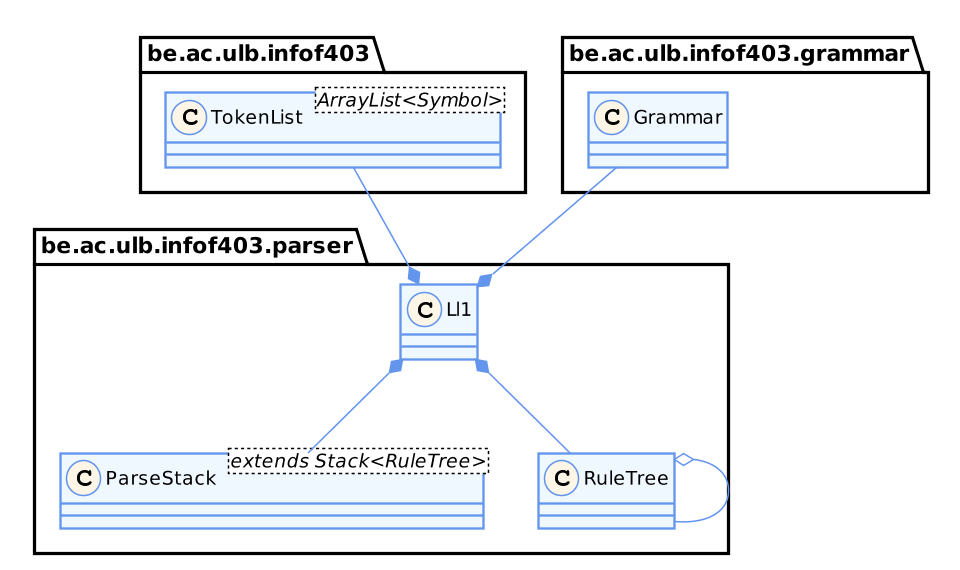
\includegraphics[scale=0.275]{./img/class_ll1.png}
      \caption{Pseudo uml of the LL1 architecture}
      \label{fig:architecturell1}
    \end{figure}
  
  \subsection{Tests and results}
    \label{sec:results}
    As previously mentioned, being able to transform a non deterministic --- but yet rather simple to write --- grammar into a implementable deterministic grammar, is something one wants to do when asked to implement a parser based on this grammar. In our case, all the methods previously presented in the section \ref{grammartoll1methods} have been applied to the IMP grammar (which is available in the annex fig.\ref{fig:basicimpgrammar}) through the use of a package containing an implemented version of these methods.\\
    The present section is composed of six subsections. The four first subsections describe and analyse the steps of \textit{LL(1)} transformation whereas the two last subsections focus respectively on the action table generated by the implementation and the results of the syntax checking.\\
    \begin{tcolorbox}
      For a matter of readability, it has been decided to only display the modified parts of the grammar. To see the full version of the modified IMP grammar one must used the process described in the subsection \ref{subsec:parameters} or must see annex fig.\ref{fig:finalimpgrammar}.
    \end{tcolorbox}
    
    \subsubsection{Ambiguity}
      Following the assignment statement, identifying the rules where ambiguity occurs is rather simple. The two ambiguous part of the grammar involved both arithmetic expressions and conditions. For both the former and the latter, atomic rules have been identified and categorised as such. Then, two layers have been introduced in order to force the derivation.\\
      In the case of arithmetic expressions, the operator $-$ has been given the highest priority. Thus it has been introduced directly in the set of atomic rules (\verb|9| to \verb|12|). After that, the $*$ and $/$ operators were given the highest priority, this is why they are part of the first layer (\verb|5| to \verb|8|). Finally, the second and last layer (\verb|1| to \verb|4|) is composed of the rules involving the remaining operators ($+$ and $-$).\\
      Notice that, even though it has not been explicitly specified in the assignment statement, any arithmetic expressions surrounded by parenthesis has been considered as having a priority as high has the $-$ operator.
      \begin{lstlisting}
<ExprArith>	     -> <ExprArith> <OpAdd> <ExprArithMul> 
<ExprArith>	     -> <ExprArithMul> 
<OpAdd>	         -> + 
<OpAdd>	         -> - 
<ExprArithMul>	 -> <ExprArithMul> <OpMul> <ExprArithAtom> 
<ExprArithMul>	 -> <ExprArithAtom> 
<OpMul>	         -> * 
<OpMul>	         -> / 
<ExprArithAtom>	 -> VarName 
<ExprArithAtom>	 -> [Number] 
<ExprArithAtom>	 -> ( <ExprArith> ) 
<ExprArithAtom>	 -> - <ExprArithAtom>\end{lstlisting}
      The same modifications have been applied on conditions than on arithmetic expressions.
      \begin{lstlisting}
<Cond>	         -> <Cond> or <CondAnd> 
<Cond>	         -> <CondAnd> 
<CondAnd>	       -> <CondAnd> and <CondAtom> 
<CondAnd>	       -> <CondAtom> 
<CondAtom>	     -> not <SimpleCond> 
<CondAtom>	     -> <SimpleCond> 
<SimpleCond>     -> <ExprArith> <Comp> <ExprArith> 
<Comp>	         -> = 
<Comp>	         -> >= 
<Comp>	         -> >  
<Comp>	         -> <=  
<Comp>	         -> <  
<Comp>	         -> <>\end{lstlisting}

    \subsubsection{Useless symbols removal}
      The unambiguous IMP grammar does not contain any useless symbols. One can be easily convinced of the reachability by drawing a graph were every variable is represented by a node and every edge represents the fact that a variable appears at least once in one the rules of the other. One can also be convinced of the grammar productiveness by observing that for each recursive rule, there is another that stops the recursivity. These intuitions were proved right by the implementation.
      
    \subsubsection{Left-recursion removal}
      When one wants to remove the left-recursion, one knows, following the definition given above, that one has to look for rules where the left-hand side is also the first element of the right-hand side.\\
      Doing so on the unambiguous and useless symbols free IMP grammar returns once again the arithmetic expressions and the conditions. But this is not surprising given the trick used to make the grammar unambiguous. This partly explains the reasons behind the order of the steps.\\
      In both cases, there are the introduction of a suffixed U variable and a suffixed V variable. These variables are respectively used to remove indirect left-recursion and to transform each direct left-recursion into a right-recursion. Notice that the introduced right-recursion are productive as the algorithm stipulates that the suffixed V variable must own an epsilon-rule\footnote{\label{epsilonrule}a variable rule which is only composed of an epsilon ($\epsilon$)}. (see lines 4 and 8 of the following grammars)
      \begin{lstlisting}
<ExprArith>	     -> <ExprArithU> <ExprArithV>
<ExprArithU>	   -> <ExprArithMul>
<ExprArithV>	   -> <OpAdd> <ExprArithMul> <ExprArithV> 
<ExprArithV>	   -> eps
<ExprArithMul>	 -> <ExprArithMulU> <ExprArithMulV>
<ExprArithMulU>	 -> <ExprArithAtom> 
<ExprArithMulV>	 -> <OpMul> <ExprArithAtom> <ExprArithMulV> 
<ExprArithMulV>	 -> eps\end{lstlisting}
      \begin{lstlisting} 
<Cond>	         -> <CondU> <CondV>
<CondU>	         -> <CondAnd> 
<CondV>	         -> or <CondAnd> <CondV> 
<CondV>	         -> eps
<CondAnd>	       -> <CondAndU> <CondAndV>
<CondAndU>	     -> <CondAtom> 
<CondAndV>	     -> and <CondAtom> <CondAndV> 
<CondAndV>	     -> eps\end{lstlisting}

    \subsubsection{Factorisation}
      Looking in a grammar for rules to factorise consists in identifying variables that have two or more rules that share a common prefix (i.e. a same sequence of tokens). Theses rules are then modified following the mechanism explained in the subsection \ref{sec:factorisation}.\\
      In the case of the unambiguous, useless symbols free and left-recursion free IMP grammar, only three variables need to see their rules factorised : \verb|InstList|, \verb|If| and \verb|For| (respectively line 4, 22 and 37 in fig.\ref{fig:basicimpgrammar}).
      \begin{lstlisting}
<InstList>	     -> <Instruction> <InstList'> 
<InstList'>	     -> ; <InstList> 
<InstList'>	     -> eps\end{lstlisting}
      The factorisation of \verb|InstList| is an instance of the particular case mentioned in subsection \ref{sec:factorisation}. In fact, one of the rules to be factorised does not really diverge as it equals the suffix. Thus an epsilon-rule$^{\ref{epsilonrule}}$ is introduced (rule 3).
      \begin{lstlisting}
<If>	           -> if <Cond> then <Code> <If'> 
<If'>	           -> else <Code> endif 
<If'>	           -> endif\end{lstlisting}
      \begin{lstlisting}
<For>	           -> for VarName from <ExprArith> <For'> 
<For'>	         -> by <ExprArith> to <ExprArith> do <Code> done 
<For'>	         -> to <ExprArith> do <Code> done\end{lstlisting}
      The factorisation of \verb|If| and \verb|For| is quite mainstream as they present a real divergence. Thus after the prefix,  a new variable is introduced and associated to the remaining of the common prefixed rules.
      
    \subsubsection{Resulting action table}
      The last tool required before starting to check the syntax of the input is the action table. Based on the final grammar obtained using the implementation and the function $first(\alpha)$ and $follow(\alpha)$, the action displayed in the annexe \ref{impactiontable} has been obtained. At the first look, the content of the action table might seems weird but everything is logic.\\
      Firstly, the variables \textit{<Print>}, \textit{<Read>}, \textit{<Program>}, \textit{<Assign>}, \textit{<While>}, \textit{<If>} and \textit{<For>} have only one filled cell. This can easily be explained as they all own only one rule that starts with a terminal. Thus nothing else than this terminal can be observed during the parsing. In the case of \textit{<If>} and \textit{<For>}, it was expected as it was meant after the factorisation. Notice that, as expected regarding the results of the factorisation, the two derived variables \textit{<If'>} and \textit{<For'>} both have two cells filled. On the other hand, \textit{<InstList'>} has more than to two cells filled (actually five) due to the introduced $\epsilon$.\\
      Secondly, the terminals \textit{:=} and \textit{from} have no filled cells due to the place in which they appear in the grammar : never as the first element of a rule and always preceded by an other terminal (\textit{VarName} for both) which explains why even $follow(\alpha)$ cannot reach them.\\
      Finally, \textit{begin} is the only terminal that has one filled cell and it is not surprising as it only appears at the first element of the only rule of the initial variable of the grammar (cannot be reach by $follow(\alpha)$).
    
    \subsubsection{Syntax checking results}  
      After having used three different source codes to test the lexical analyser (subsection \ref{subsec:testscanner}), we use them to assess the parser.\\
      Firstly, \verb|Euclid.imp| (fig.\ref{code:euclid}) totally respects the syntax defined by the final IMP grammar and requires 120 transitions (matches excluded).\\ % TODO transition correct ??
      Secondly, \verb|Fibonacci.imp| (fig.\ref{code:fibonacci}) also respects the syntax and requires 85 transitions (matches excluded). During the very first test of the parser on \verb|Fibonacci.imp|, we encountered an error and then realised that the first version (written during the realisation of first part of the project) contained an error. In fact, the instruction line 11 ended with a semicolon and thus did not respect the grammar (more precisely the rule 52 of the final grammar (annex fig.\ref{fig:finalimpgrammar})). Despite being counter intuitive for a programmer, this rule helped us ensuring the well functioning of the parser.
        \begin{verbatim}
(line : 12 col :4)	Unexepected character 'done' of type DONE
    The expected character is one of the following : while if print VarName for read
        \end{verbatim}
    Finally, as expected, \verb|Sort.imp| (fig.\ref{code:sort}) is not even parsed as an error occurs during the scanning. Hence, the compiler will display the following message~:
      \begin{verbatim}
Error with a token: Unknown symbol '[' (9 character at line 1)
      \end{verbatim}
      
\section{Implementation of the semantic analyser}

  \subsection{Use and implementation of the compiler generator}
    \begin{figure}[h!]
      \centering
      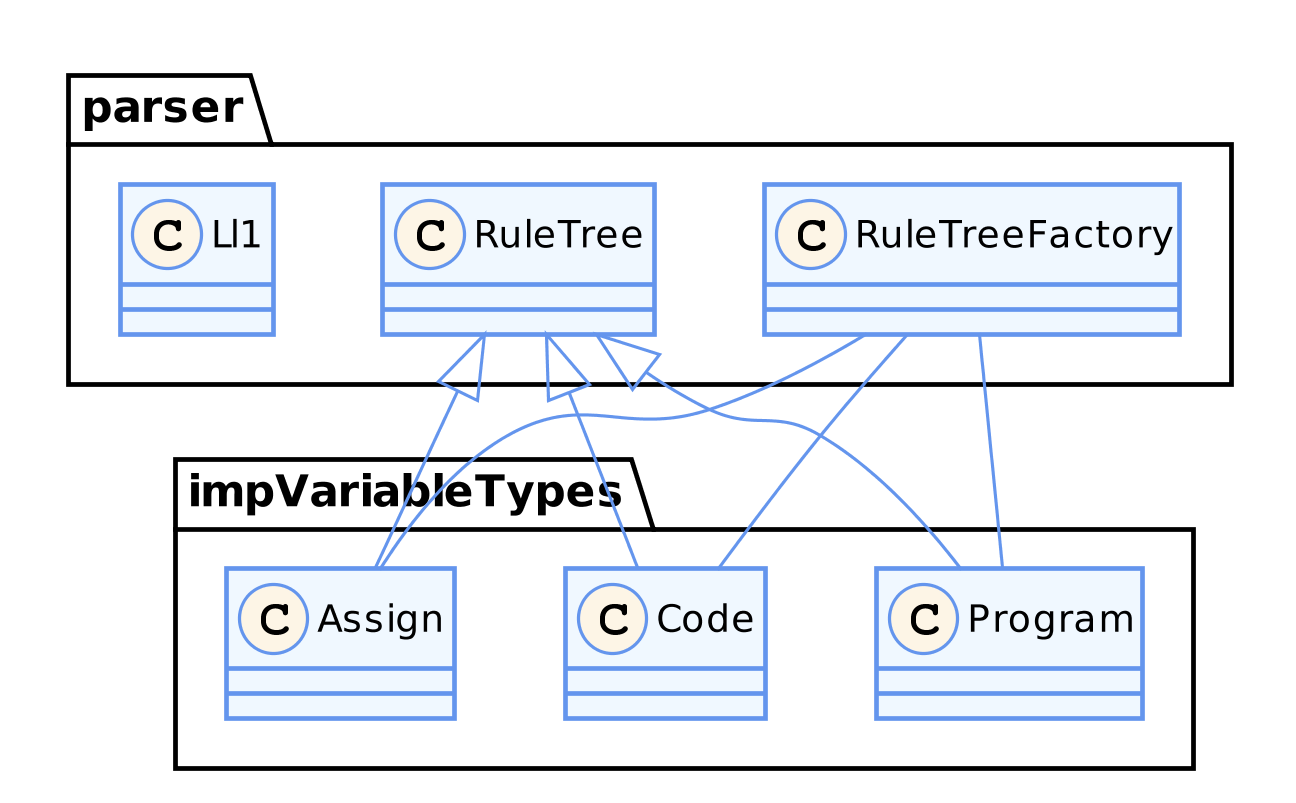
\includegraphics[scale=0.175]{img/class_ruleTree.png}
    \end{figure}

  
  \subsection{How the project generates LLVM code}
    Like mention in the section \ref{sec:resulting_parser}, the parse tree is composed by \verb|RuleTree| object. We have create a children of this class for each state of the grammer. To generate the LLVM code we just make recursive call. Indeed the first state \verb|Program| call the result of \verb|Code|.  Which call the result of the instruction, ect.\\
    When a state compute his result he could also ``output'' LLVM code (this output is first store in varable and then output on the right support: file or terminal). In other words, children of \verb|RuleTree| have a method which return the value that represent the current state \textbf{and} output an LLVM code to compute this value.\\
    This method work for a lot of state. There are just some problem with the addition structure. The figure \ref{fig:addition_states} show us that the state \verb|ExprArithMulV| have not all element to compute the division. To fix that there are two choice: get the missing value from the parent or compute the division on another state. We chose to implement the second option.  Thus the state \verb|ExprArithMul| will compute the result of the division and store this value on a new variable.\\
    To make that the state \verb|ExprArithMul| will get the operator with two get: one on his second children and then directly ask to get the value of the first children. To have the value 4 (in this case), \verb|ExprArithMul| will ask at state \verb|ExprArithMulV| to compute his final value.  Then, \verb|ExprArithMul| have all element to compute the division.
    
    \begin{figure}[h!]
      \centering
      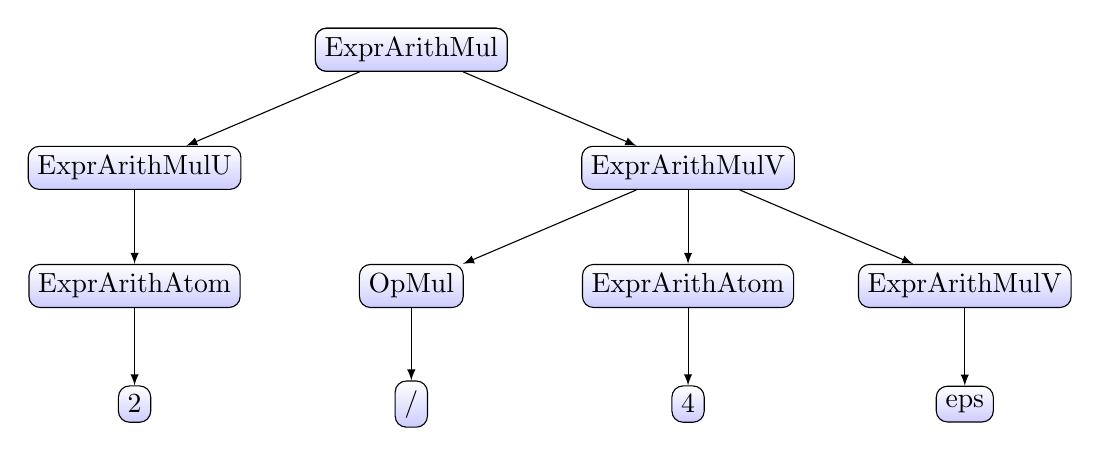
\begin{tikzpicture}[tree,sibling distance=20em,level 2/.style={sibling distance=10em}]
	\node {ExprArithMul}
	node {ExprArithMul}
	  child {
	    node {ExprArithMulU}
	      child {
		node {ExprArithAtom}
		  child {
		    node {2}
		  }
	      }
	  }
	  child {
	    node {ExprArithMulV}
	    child {
	      node {OpMul}
		child {
		  node {/}
		}
	    }
	    child {
	      node {ExprArithAtom}
		child {
		  node {4}
		}
	    }
	    child {
	      node {ExprArithMulV}
		child {
		  node {eps}
		}
	    }
	  };
      \end{tikzpicture}
      \caption{Part of parse tree which compute Expression.}
      \label{fig:addition_states}
    \end{figure}
    
  \subsection{Limitations}
    \label{semantic-limitations}
    Even though the mechanism used to generate the \textit{LLVM} code was simple to simple to implement, not transforming the \textit{parse tree} returned by the \textit{syntax analyser} into an \textit{Abstract Syntax tree} or another structure disabled us from using many optimisation techniques mentioned in the assignment statement.\\
    The most obvious consequence is that it is impossible to implement a mechanism that evaluates the arithmetic expressions for which the involved variables value is already known at the compilation time. This has for consequence that useless code is generated by the compiler and that the resulting executable will be heavier than what might be achieved. Hopefully, the \textit{LLVM} compiler/interpreter implements this features.
  
  \subsection{Hypothesis}
    Throughout the project, only one hypothesis has been settled. This hypothesis is the following~: when using the rule
    \begin{verbatim}
      for varName from <ExpreArith> by <ExpreArith> to <ExpreArith> do <Code> done
    \end{verbatim}
    the first \verb|<ExpreArith>| has to be \underline{strictly} lower than the third \verb|<ExpreArith>| and the second \verb|<ExpreArith>| has to be greater or equal than $0$ (even if incrementing by $0$ does not make any sense).\\
    This issue arises because, unlike c/c++, the programmer does not have to explicitly specify the condition. Thus, the compiler has to be able to decide by itself whether a $>$ or $<$ operator should be used. This would imply that the compiler should be able to evaluate its arithmetic expressions during the \textit{compilation time} but this is not possible as mentioned above (see section \ref{semantic-limitations}). Further more, if the arithmetic expressions of the \verb|for| involve a varibale that is modified in the instruction block, no evaluation is possible. In sum, no decision over the operator to used can be taken.
  
  \subsection{Results}
    

\section{How to set up the project}
  In order to simplify the compilation and the support of external libraries, it has been decided to use a well known \textit{java} project manager named \textit{Maven}. Its configuration file (\verb|pom.xml|) defines the \verb|main| file, defines the source folder, manages the \textit{JFlex} library and the package that must be compiled with this library.
  \subsection{Compilation}
    Compiling the project with \textit{Maven} is easy as the user only needs to execute~: \verb|mvn clean compile|. However, at the first execution, the user needs to execute \verb|mvn install| so that \textit{Maven} can install the required library.\\
    If the user does not want to use \textit{Maven}, he can execute different commands from the root project~:
    \begin{lstlisting}[numbers=none,backgroundcolor=,basicstyle=\small\ttfamily]
java -jar jflex-1.6.1.jar -d src/be/ac/ulb/infof403/scanner/ src/be/ac/ulb/infof403/lex/Scanner.flex
java -jar jflex-1.6.1.jar -d src/be/ac/ulb/infof403/grammar/ src/be/ac/ulb/infof403/lex/GrammarScanner.flex
    \end{lstlisting}
    Where \verb|jflex-1.6.1.jar| is the path to the \verb|.jar| executable library,  \verb|-d| is the output folder path specifier and the last parameter is the path to the \verb|.flex| file.\\
    Then, the user can compile the java source codes and can create the corresponding \verb|.class| files. The bash command to compile all the \textit{java} files located in the \verb|src/| folder is the following~:
    \begin{verbatim}
javac -d target $(find ./src/* | grep .java)
    \end{verbatim}
    This command generates the corresponding \verb|.class| files and put them in the \verb|target/| folder. The user must create the "target" folder if it does not currently exist. Finally, the \textit{jar} file can be generated by using the command~:
    \begin{verbatim}
jar cvfe dist/INFO-F403-IMP.jar be/ac/ulb/infof403/Main -C target/ .
    \end{verbatim}
    Where \verb|INFO-F403-IMP.jar| is the name of the generated \textit{jar} file and \textit{target} is the folder where the \verb|.class| files are located.
    
  \subsection{Execution}
    To execute the resulting jar file, the user only has to type~:
    \begin{verbatim}
java -jar dist/INFO-F403-IMP.jar <grammarFile> <IMPFile>
    \end{verbatim}
    Where \verb|<IMPFile>| is the path to the IMP file (by default: \verb|./test/imp/Euclid.imp|) and \verb|<grammarFile>| is the path to the Grammar used to parse IMP file (by default: \verb|./test/grammar/UnambiguousIMP.gram|).
    
  \subsection{Test}
    \label{subsec:test}
    % TODO remy j'ai pas compris ce que tu veux dire en utilisant instruction
    Maven contains instruction to automatically make some test.  If the user wants to execute these tests, he must execute this command: \verb|mvn verify|. The user can execute the tester using the compilation command~: \verb|mvn verify clean compile|.\\
    There are not lot of tests but it's easy to create more. Tests are located in the folder \verb|srcTest/|. 
    It's also possible to test the IMP scanner. Indeed, the user can see the outcome of the scanning of the IMP file by adding the argument \verb|--printscan| (or the alias \verb|-ps|) and can compare this output to an existing ``\verb|.out|`` file. To do so, the user needs to add the argument \verb|--testscan| (or the alias \verb|-ts|) followed by the expeted output file.\\
    To summarize, you could execute:
    \begin{verbatim}
java -jar dist/INFO-F403-IMP.jar -ps -ts test/imp/Euclid.out\end{verbatim}
    Note that if the user does not specify the expected output file, the program will automatically load a test file based on the \textit{source file} name.
    
  \subsection{Javadoc}
    The javadoc is located in the \verb|doc/| folder. To generate the javadoc with Maven the user must execute \verb|mvn javadoc:javadoc|.  If he does not want to user Maven, he can execute the following command~:
    \begin{verbatim}
javadoc -d doc/javadoc/ -keywords -sourcepath src -subpackages be
    \end{verbatim}
    Where \verb|doc/javadoc/| is the output folder. The option \verb|-keywords| enables HTML in the javadoc.
    
  \subsection{Parameters}
    \label{subsec:parameters}
    The user can see all the parameters by using the argument \verb|--help| (or the alias \verb|-h|).  If he wants to analyse a specific IMP file he \textbf{must} precise the grammar file first. There is no order for the other arguments. The user will find bellow the list of possible arguments:
    \begin{itemize}
      \item \verb|-h/--help| Displays all arguments
      \item \verb|-ta/--table| Prints the action table (see point \ref{subsubsec:actionTable})
      \item \verb|-ts/--testscan| Checks that the result of the scan is the same that the expected output (see point \ref{subsec:test}).
      \item \verb|-ps/--printscan| Prints the scan result (used to compare with the ''.out`` file (if specified with previous argument)).
      \item \verb|-gojs/--gojstree| Displays the parse tree using GoJS library.
      \item \verb|-tex/--latex| Displays the parse tree in a \LaTeX\ format. (Note: this method uses the Tikz library and big trees cannot be compiled).
      \item \verb|-d/--debug| Displays a lot of debug messages (used to develop)
    \end{itemize}
    
\newpage
\appendix
\addtocontents{toc}{\protect\setcounter{tocdepth}{1}}

\section{Annex}
  \subsection{Grammar factorisation}
    \label{sec:factorisation}
    This mechanism is applied every time a given variable has two (or more) rules with a common prefix. The aim is to reduce the number of repetitions. To achieve this, each variable that has two (or more) rules with a common prefix sees these rules replaced by concatenation of the prefix and a new variable. This new variable has for rules the remaining of the factorized rules (i.e. the rules that have a common prefix without this prefix).
    \begin{figure}[h!]
	  \begin{subfigure}[b]{0.4\textwidth}
	      \centering
	      \begin{align}
		S &\rightarrow friendship \\
		  &\rightarrow friend \\
		  &\rightarrow relationship \\
		  &\rightarrow friendly
	      \end{align}
	      \caption{Unmodified grammar}
	      \label{fig:unmodifiedgrammar1}
	  \end{subfigure}%
	  \begin{subfigure}[b]{0.4\textwidth}
	      \centering
	      \begin{align}
		S  &\rightarrow relationship \\
		    &\rightarrow friendS' \\
		S' &\rightarrow ship \\
		    &\rightarrow ly \\
		    &\rightarrow \epsilon
	      \end{align}
	      \caption{Factorisation outcome}
	      \label{fig:resultinggrammar1}
	  \end{subfigure}
	  \caption{Left-factorisation example}
      \end{figure}\\
      For instance, in the fig.\ref{fig:unmodifiedgrammar1}, the rule (7) has no prefix whit the other rules whereas (5), (6) and (8) have a common prefix : '\textit{friend}'. Thus, following the mechanism explained above, we replace these three rules by a new one (rule (10)) composed of the prefix ('\textit{friend}') and the new variable (\textit{S'}). The variable \textit{S'} is then associated whit the remaining of each former rule with a common prefix of \textit{S}. Notice that the rule (6) is a particular case as it matches exactly the prefix. To overcome this issue, the created rule is formed of $\epsilon$ (rule (13)).\\\\
      Such a technique is used to ensure that the parser will be deterministic. In our case, we want to implement a parser with a look ahead of one. Therefore, if a variable has two (or more) rules like $S \rightarrow fA$ and $S \rightarrow fZ$, the parser won't be able to decide which one to apply.

  \subsection{Removing left-recursion}
    \label{sec:leftrecursion}
    Even though recursion is a main feature of grammars as it allows them to recognise non-finite languages, it also introduces non-determinism when the recursion occurs at the very first element of the right-hand side. To make a grammar (and thus the parser) deterministic while keeping the recursivity, one must execute to manipulations.
    \begin{figure}[h!]
      \centering
      \begin{subfigure}[b]{0.33\textwidth}
	  \centering
	  \begin{align}
	    S  &\rightarrow S'b \\
	    S' &\rightarrow Sa \\
		&\rightarrow \epsilon
	  \end{align}
	  \caption{Unmodified grammar}
	  \label{fig:unmodifiedgrammar2}
      \end{subfigure}%
      \begin{subfigure}[b]{0.33\textwidth}
	  \centering
	  \begin{align}
	    S  &\rightarrow Sab \\
		&\rightarrow b
	  \end{align}
	  \caption{Indirect recursion removal}
	  \label{fig:indirectremovalgrammar2}
      \end{subfigure}
      \begin{subfigure}[b]{0.33\textwidth}
	  \centering
	  \begin{align}
	    V  &\rightarrow bV' \\
	    V' &\rightarrow abV' \\
		&\rightarrow \epsilon
	  \end{align}
	  \caption{Transformation to right-recursive}
	  \label{fig:rightrecursivegrammar2}
      \end{subfigure}
      \caption{Left-recursion removal example}
    \end{figure}\\
    First, one wants to transform every indirect left-recursion into direct left-recursion. Achieving that is quite simple as one only has to take a rule and replace the variable located at the very beginning of the left-hand side and replace it by all of its own rules. For instance, in fig.\ref{fig:unmodifiedgrammar2}, the grammar is indirectly recursive because \textit{S} calls \textit{S'} which, when applying rule (15), calls \textit{S}. The out come of this transformation (see fig.\ref{fig:indirectremovalgrammar2}) recognises the same language but is now directly left-recursive.\\
    Secondly, one wants to transform every left-recursion by a right-recursion for determinism purpose (similar to factorisation). One can achieve it by introducing two new variables. The first variable will be associated to a set of rules each composed of the concatenation of a non-recursive rule and the newly created second variable. This second variable will be associated with a set of rules composed of every recursive rules where the first element (the recursive variable)has been removed concatenated with this exact second variable. Doing so transforms every left-recursion in a right-recursion. However, this right-recursion will never stops. This is why a rule composed of $\epsilon$ is associated to the second variable.

  \subsection{Removing useless variables}
    \label{sec:useless}
    When speaking of \textit{useless} variables, we distinguish two types of variables~:
    \begin{description}
      \item[The \textit{unproductive} ones~:]
  An unproductive variable is a variable that never leads to any formation of a word. Typically, such a variable does not have any non-recursive rule. Thus, forming a word using this variable leads to an infinite recursion.
      \item[The \textit{unreachable} ones~:]
  An unreachable variable is a variable that is not called by any other rule of the grammar in which it belongs.
    \end{description}
    So far, the best way to find both unproductive and unreachable variables is to look respectively for productive and reachable variables and remove them from the grammar afterwards. However, eventually, we are only interested in productive and reachable variables. Thus, once the former and the latter are found, we consider them as the final grammar.\\\\
    Determining the set of productive symbols consists of first considering every terminal as productive. Then, for each variable, we look at each rule and add the variable to the set if and only if every symbols appearing in the rule are already in the set. The resulting set is the set of every reachable symbols of the given grammar.\\\\
    % Add an example.
    Retrieving the set of reachable symbols from a given grammar can be achieved by using a similar method to the one explained above. In fact, one must consider first a set containing only the initial variable of the grammar which is --- without lost of generality --- always considered as reachable. Then, for each variable of the grammar, one must check whether the variable is in the set of reachable symbols. If yes, one can then add all the symbols appearing in the rules of this variable.
    
  \subsection{Ambiguous grammar}
    \label{sec:ambiguity}
    Ambiguity occurs when, for a given word/input, multiple interpretations (or trees) can be derived due to a multiple choice of rules, leading the parser to take a non-deterministic choice and thus make it not adapted for implementation. Unfortunately, there does not exist any algorithm resolving this issue as the given grammar gives little information. Henceforth, extra information only known by the language designer must be integrated. The most common example of ambiguity is the arithmetic priority (Reminder : the multiplication has an higher priority than the addition).
      \begin{figure}[h!]
	\centering
	\begin{subfigure}[b]{0.4\textwidth}
	    \centering
	    \begin{align}
	      Exp &\rightarrow Exp+Exp \\
		  &\rightarrow Exp*Exp \\
		  &\rightarrow Cst \\
		  &\rightarrow Id
	    \end{align}
	    \caption{Ambiguous grammar}
	    \label{fig:unmodifiedgrammar3}
	\end{subfigure}%
	\begin{subfigure}[b]{0.4\textwidth}
	    \centering
	    \begin{align}
	      Exp  &\rightarrow Exp+Prod \\
		    &\rightarrow Prod \\
	      Prod &\rightarrow Prod*Atom \\
		    &\rightarrow Atom \\
	      Atom &\rightarrow Cst \\
		    &\rightarrow Id
	    \end{align}
	    \caption{Unambiguous grammar}
	    \label{fig:unambiguousgrammar3}
	\end{subfigure}
	\caption{Unambiguity mechanism example}
    \end{figure}\\
    For example, applying the grammar of fig.\ref{fig:unmodifiedgrammar3} on the word $id+id*id$ will result in two different interpretation as shown in Fig.\ref{fig:ambiguoustree1} and Fig.\ref{fig:ambiguoustree2}.\\
  \begin{figure}[h!]
    \centering
    \begin{subfigure}[b]{0.4\textwidth}
      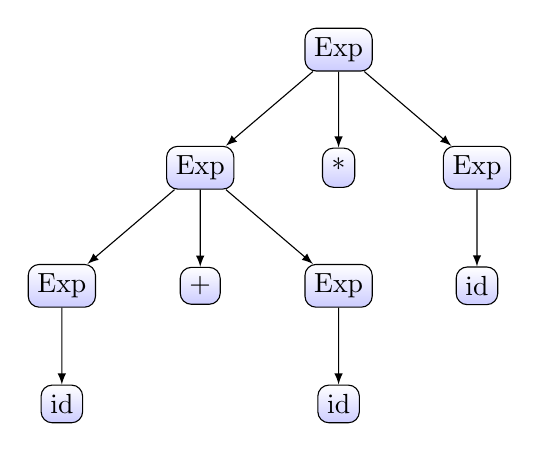
\begin{tikzpicture}[tree]
	\node {Exp}
	child {
	  node {Exp}
	child { node {Exp} 
	child { node {id} }
	}
	  child { node {+} }
	  child { 
	node {Exp}
	child { node {id} }
	  }
	}
	child { node {*} }
	child { 
	  node {Exp}
	child { node {id} }
	};
      \end{tikzpicture}
      \caption{First possible derivation of the input.}
      \label{fig:ambiguoustree1}
    \end{subfigure}
    \hfill
    \begin{subfigure}[b]{0.4\textwidth}
      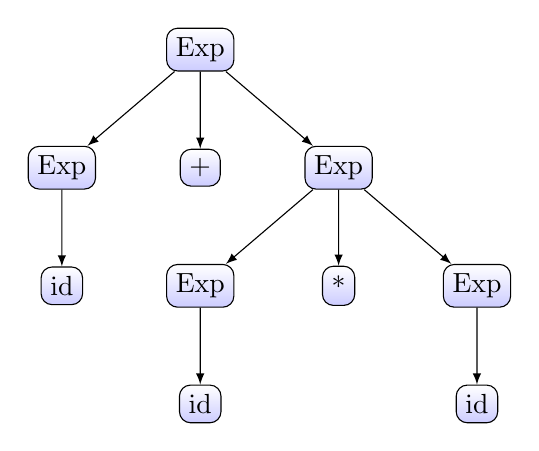
\begin{tikzpicture}[tree]
	\node {Exp}
	child { 
	  node {Exp}
	child { node {id} }
	}
	child { node {+} }
	child {
	  node {Exp}
	child { node {Exp} 
	child { node {id} }
	}
	  child { node {*} }
	  child { 
	node {Exp}
	child { node {id} }
	  }
	};
      \end{tikzpicture}
      \caption{Second possible derivation of the input.}
      \label{fig:ambiguoustree2}
    \end{subfigure}
    \caption{Derivations of the input $id+id*id$ using the grammar in fig.\ref{fig:unmodifiedgrammar3}}
  \end{figure}
  To address this issue, the language designer must 'force' the derivation (and hence the priority) by introducing new variables that could be seen as extra layers. For instance, on fig.\ref{fig:unmodifiedgrammar3}, the grammar is composed of two \textit{atomic} terminals : \textit{Cst} and \textit{Id}. These terminals will be encapsulated in a new variable called \textit{Atom}. In addition, we decide --- based on the arithmetic priority --- that multiplication has an higher priority than addition. Therefore, as for atomic elements, we introduce a new variable called \textit{Prod} that has for rules a single atomic value (29) and the product of a multiplication and a atomic element (28). Finally, the same mechanism is once again applied to addition. Resulting in the rules (26) and (27).\\
  \begin{tcolorbox}
    As previously mentioned, there does not exist an algorithm that resolves grammar ambiguity. However, there exists many ambiguity detection algorithms that have their own proprieties as listed in this article\footnote{H.J.S. Basten, August 17, 2007. \textit{Ambiguity Detection Methods for Context-Free Grammars.} Master's Thesis, Universiteit Van Amsterdam.}. The reader is invited to read this document for further information.
  \end{tcolorbox}

    \begin{figure}[h!]
      \centering
      \begin{lstlisting}
<Program>       -> begin <Code> end
<Code>          -> eps
                -> <InstList>
<InstList>      -> <Instruction>
                -> <Instruction> ; <InstList>
<Instruction>   -> <Assign>
                -> <If>
                -> <While>
                -> <For>
                -> <Print>
                -> <Read>
<Assign>        -> [VarName] := <ExprArith>
<ExprArith>     -> [VarName]
                -> [Number]
                -> ( <ExprArith> )
                -> - <ExprArith>
                -> <ExprArith> <Op> <ExprArith>
<Op>            -> +
                -> -
                -> *
                -> /
<If>            -> if <Cond> then <Code> endif
                -> if <Cond> then <Code> else <Code> endif
<Cond>          -> <Cond> <BinOp> <Cond>
                -> not <SimpleCond>
                -> <SimpleCond>
<SimpleCond>    -> <ExprArith> <Comp> <ExprArith>
<BinOp>         -> and
                -> or
<Comp>          -> = 
                -> >= 
                -> > 
                -> <= 
                -> < 
                -> <> 
<While>         -> while <Cond> do <Code> done
<For>           -> for [VarName] from <ExprArith> by <ExprArith> to <ExprArith> do <Code> done
                -> for [VarName] from <ExprArith> to <ExprArith> do <Code> done
<Print>         -> print ( [VarName] )
<Read>          -> read ( [VarName] )
      \end{lstlisting}
      \caption{The basic IMP grammar as given in the assignment statement.}
      \label{fig:basicimpgrammar}
    \end{figure}
  
  \begin{figure}[h!]
    \centering
    \lstinputlisting{../../test/grammar/FinalIMP.gram}
    \caption{The final IMP grammar after modifications.}
    \label{fig:finalimpgrammar}
  \end{figure}

  \begin{figure}
    \centering
    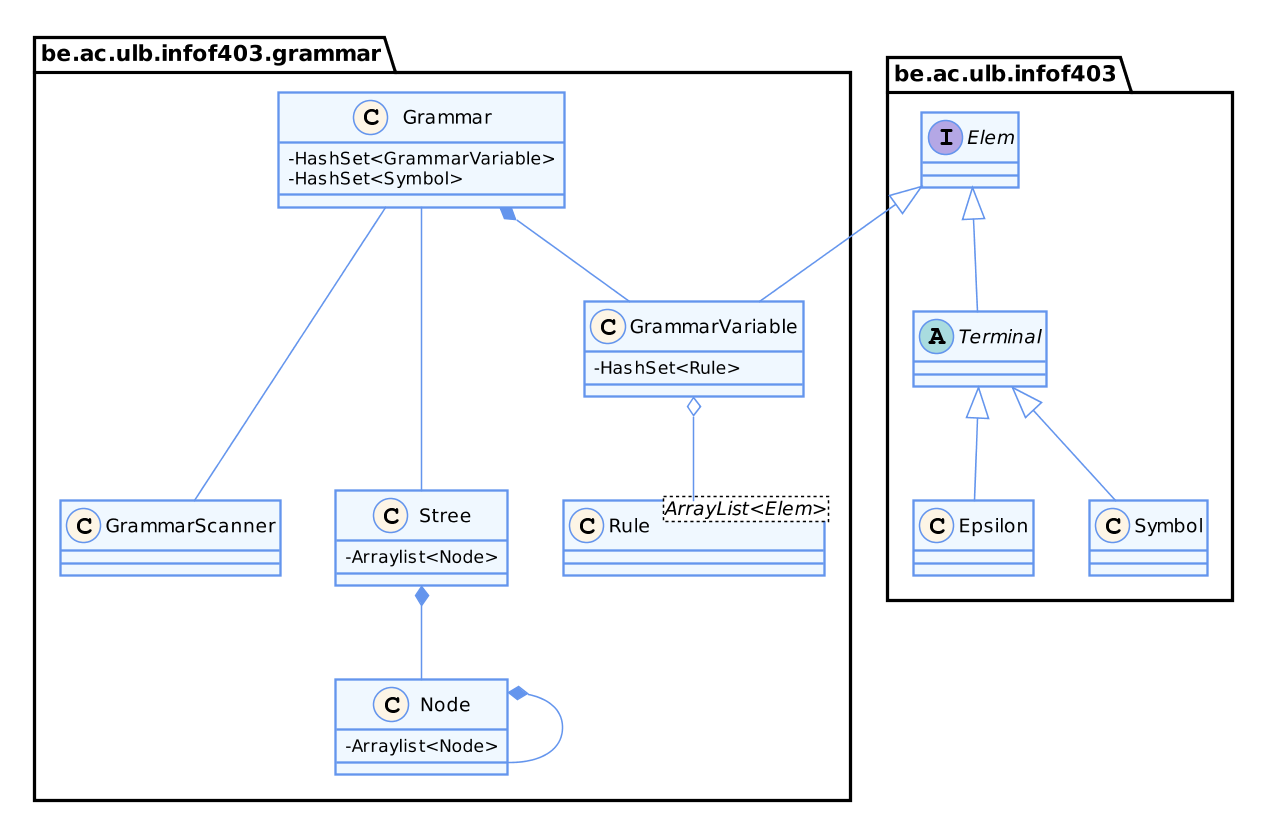
\includegraphics[width=\textwidth]{./img/class_grammar.png}
    \caption{Architecture of the grammar}
    \label{fig:grammararchitecture}
  \end{figure}
  
  \begin{sidewaystable} % <-- HERE
    \centering
    \input{ActionTable.txt}
    \caption{IMP action table.}
    \label{impactiontable}
  \end{sidewaystable}
  
  \begin{figure}[h!]
    \centering
    \lstinputlisting{../../llvm/Euclid.ll}
    \caption{The final LLVM code generation for Euclid.}
    \label{fig:finalllvmeuclid}
  \end{figure}
  
  \begin{figure}[h!]
    \centering
    \lstinputlisting{../../llvm/Fibonacci.ll}
    \caption{The final LLVM code generation for Fibonacci.}
    \label{fig:finalllvmfibonacci}
  \end{figure}
  

\end{document}
